\documentclass[final]{beamer} % beamer 3.10: do NOT use option hyperref={pdfpagelabels=false} !
% Copyright (c) 2025 Dominik Szajerman <dominik.szajerman@p.lodz.pl> Karolina Nowak <karolina.nowak@p.lodz.pl>
\mode<presentation>{\usetheme{Berlin}}
\beamertemplatenavigationsymbolsempty
%
\usepackage[main=polish,english]{babel}
\usepackage[T1]{fontenc}
\usepackage[utf8]{inputenc}
\usepackage{amsmath,amsthm,amssymb,latexsym}
\usefonttheme[onlymath]{serif}
\boldmath
\usepackage[orientation=portrait,size=custom,width=70.7,height=100.0,scale=1.45]
{beamerposter}%custom=b1%,grid,debug
\setbeamersize{text margin left=1.5cm,text margin right=1.5cm} 
\usepackage{graphicx}
\usepackage{subcaption}
\usepackage[super]{nth}
\usepackage{lipsum}
\usepackage{ragged2e}
\usepackage[none]{hyphenat}
\sloppy

\setbeamertemplate{headline}{%
        \vspace{1.5cm}%
        \hspace{1.5cm}%
        
\includegraphics[height=6.1cm]{figures/logo-pl-institute.png}\hfill%
        
\includegraphics[height=4.7cm]{figures/logo-ftims.png}\hfill%
        
\includegraphics[height=5.3cm]{figures/logo-ibd.png}\hfill%
        
\includegraphics[height=4.2cm]{figures/logo-dd.png}%
        \hspace{1.5cm}
 }
\addtobeamertemplate{footline}{}{\vskip1.75cm}
\definecolor{PLcolor}{rgb}{0.475, 0.102, 0.125}
\usecolortheme[named=PLcolor]{structure}

\title[\hspace{1cm} Petify – aplikacja wspierająca adopcję zwierząt]{Petify – aplikacja wspierająca adopcję zwierząt}

\author[\hspace{1cm} Mikołaj Bartosiak, Jakub Hynasiński, Mateusz Kołata, Jan Rzepkowski, Wiktor Szewczyk, Piotr Tomalak]{Mikołaj Bartosiak, Jakub Hynasiński, Mateusz Kołata, Jan Rzepkowski, Wiktor Szewczyk, Piotr Tomalak}

\institute[Instytut Informatyki, Politechnika Łódzka, al. Politechniki 8, 93-590 Łódź \hspace{1cm}]{Instytut Informatyki, Politechnika Łódzka}

\date{12 czerwca 2025}

\graphicspath{ {figures/} }

\begin{document}
\renewcommand{\abstractname}{Streszczenie}
\renewcommand{\figurename}{Rysunek}
\renewcommand{\tablename}{Tabela}
\captionsetup[figure]{labelformat=simple, labelsep=colon, font=small}
\renewcommand\thesubfigure{Rysunek \arabic{subfigure}}
\begin{frame}{}
\maketitle
%\vfill
\begin{abstract}
\centering
Petify to innowacyjna platforma odpowiadająca na problem bezdomności zwierząt w Polsce. Aplikacja usprawnia proces adopcji dzięki prostemu i przyjaznemu interfejsowi do przeglądania profili zwierząt. Użytkownicy mogą przeglądać zdjęcia i opisy zwierząt, stosować filtry geolokalizacyjne oraz bezpośrednio kontaktować się ze schroniskami.
System składa się z aplikacji mobilnej do dynamicznego przeglądania profili oraz aplikacji webowej z panelem administracyjnym dla schronisk.
Petify nie tylko ułatwia znalezienie pupila, ale również buduje trwałe relacje między schroniskami, wolontariuszami i~adoptującymi, czyniąc adopcję początkiem wspólnej przygody.
\end{abstract}

\begin{columns}[T]
\begin{column}[T]{0.48\textwidth}
\begin{block}{Wstęp}
\justifying
Według najnowszego raportu Głównego Lekarza Weterynarii w 2022 roku w 226 polskich schroniskach przebywało łącznie 84 008 psów oraz 34 050 kotów – razem ponad 118 tys. zwierząt.
W ciągu roku nowy dom znalazło 53 503 psów (63,7\%) i 20 345 kotów (59,8\%), jednak w klatkach nadal pozostało niemal 33 tys. czworonogów.
Statystyki te od dekady utrzymują się na alarmująco wysokim poziomie, a możliwości promowania adopcji wciąż opierają się głównie na statycznych ogłoszeniach i profilach w mediach społecznościowych.

\begin{figure}[h]
\centering
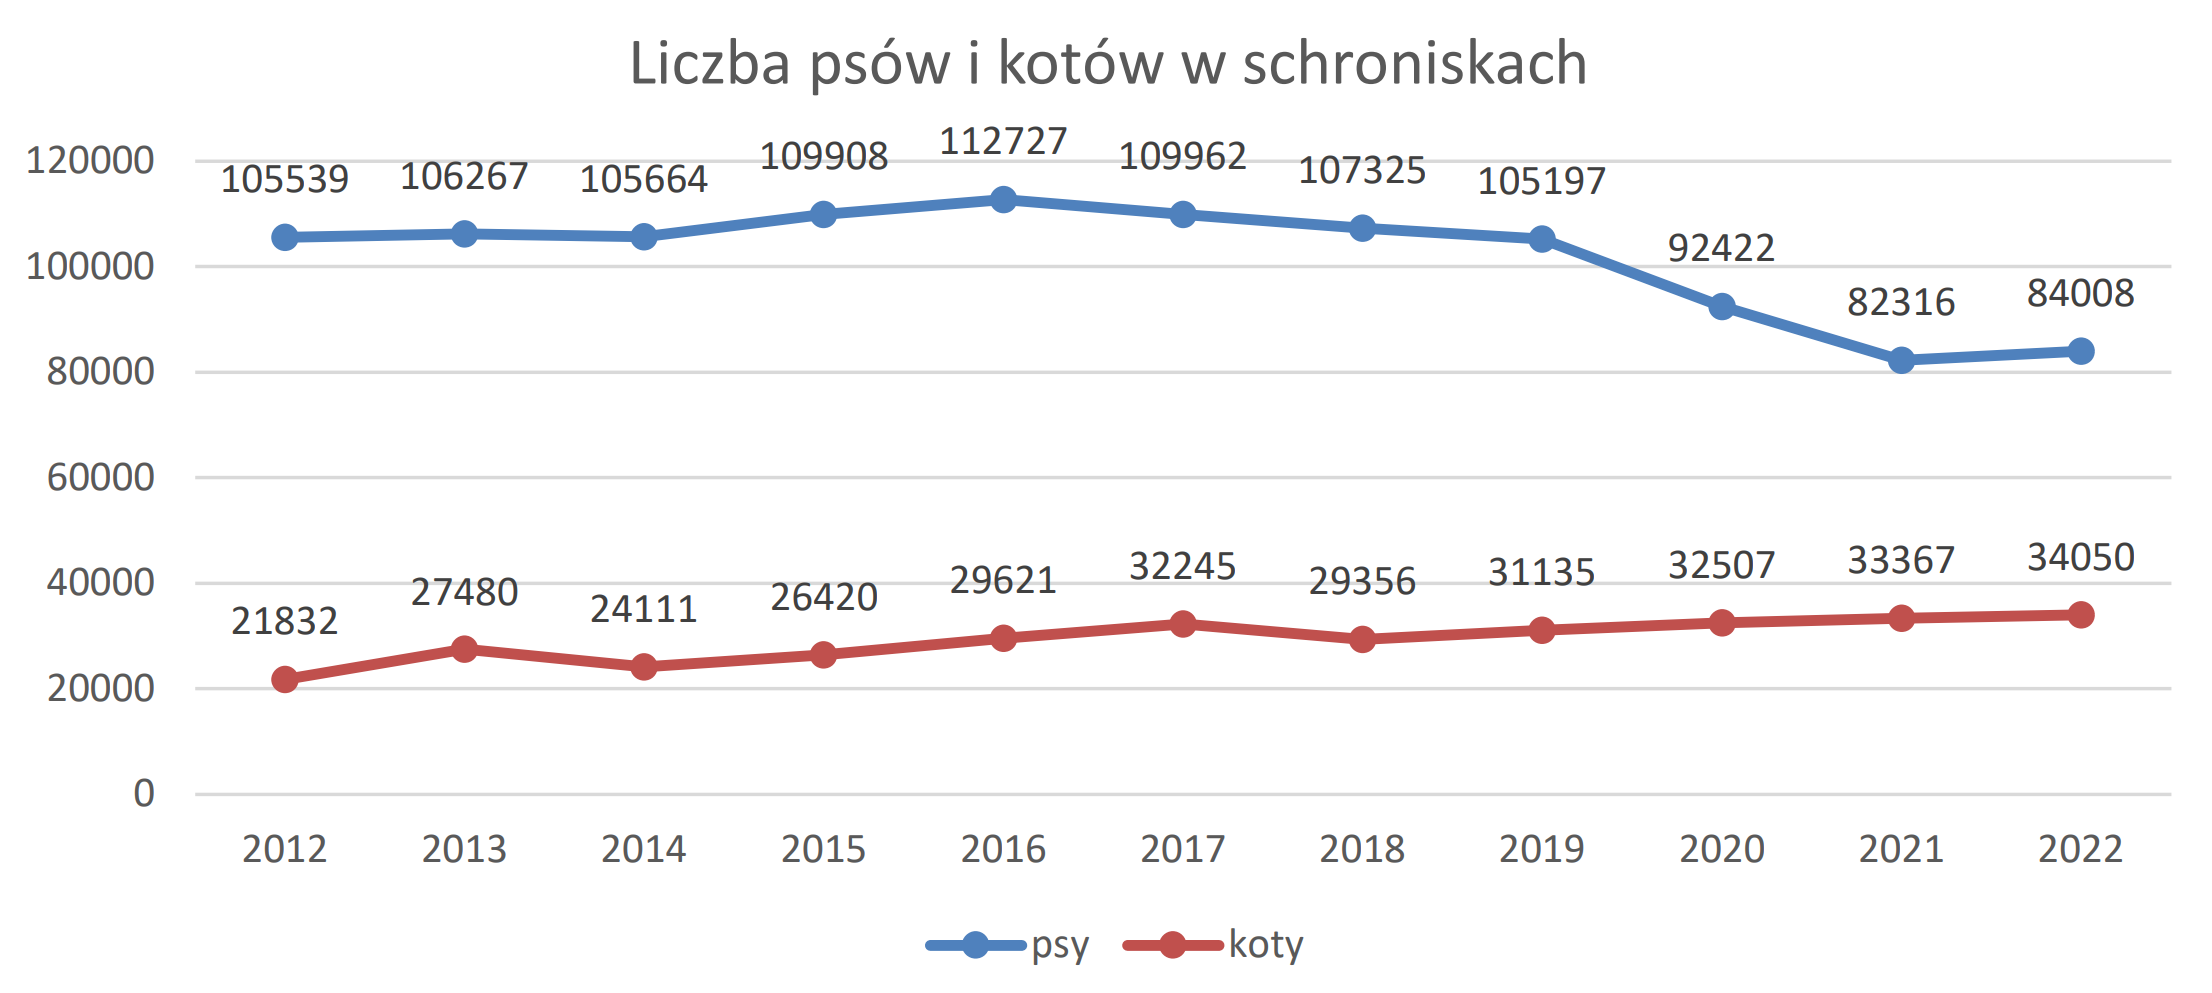
\includegraphics[width=1.0\textwidth]{chart.png}
\caption{Liczba zwierząt w polskich schroniskach w latach 2012-2022.}
{\centering\small Źródło: \itshape{https://shorturl.at/Q3W6p}\par}
\label{fig:chart}
\end{figure}
Schroniska, zmagające się z niedoborem funduszy, personelem działającym na granicy możliwości i ciągłą koniecznością poprawy warunków, potrzebują narzędzia, które wykorzysta nowoczesne technologie do połączenia opiekunów i zwierząt w bardziej intuicyjny i angażujący sposób.

\end{block}
\begin{block}{Projekt aplikacji}
\justifying
Platforma Petify składa się z dwóch uzupełniających się aplikacji, które korzystają z~architektury mikroserwisowej opartej na Java Spring Boot i~bazie danych PostgreSQL.

\textbf{Aplikacja mobilna (Flutter)} działająca natywnie na systemach Android oraz iOS, jest przeznaczona dla użytkowników i~wolontariuszy. Pozwala szybko przeglądać profile zwierząt, korzystać z~filtrów lokalizacyjnych, nawiązywać bezpośredni kontakt ze schroniskiem i~jednym dotknięciem zgłaszać chęć adopcji lub pomocy.

\textbf{Aplikacja webowa (React)} jest dostępna dla wszystkich, ale wyróżnia się rozszerzonymi funkcjami dla schronisk i~zespołu administracyjnego. Oprócz standardowego przeglądania ogłoszeń i~składania wniosków adopcyjnych udostępnia panel do tworzenia i~aktualizowania ogłoszeń, zarządzania profilami zwierząt oraz pełnego monitorowania przebiegu adopcji.

Wspólny backend zapewnia spójność danych w czasie rzeczywistym, umożliwiając użytkownikowi płynne przechodzenie między aplikacją mobilną a~wersją przeglądarkową.
\end{block}
\end{column}
\begin{column}[T]{0.48\textwidth}
\begin{block}{Implementacja}
\justifying
Po uruchomieniu aplikacji użytkownik zostaje przeniesiony do ekranu z~przewijaną listą dostępnych zwierząt. Każde zwierzę prezentowane jest na dużym zdjęciu wraz z~imieniem, wiekiem, rasą i~odległością od użytkownika. Profile można przesuwać w~lewo, aby pominąć, lub w~prawo, aby dodać zwierzaka do polubionych. Dedykowany przycisk umożliwia przekazanie wsparcia finansowego dla wybranego pupila.
\vspace{0.2cm}
\begin{figure}[h]
\centering
\begin{subfigure}{0.325\textwidth}
    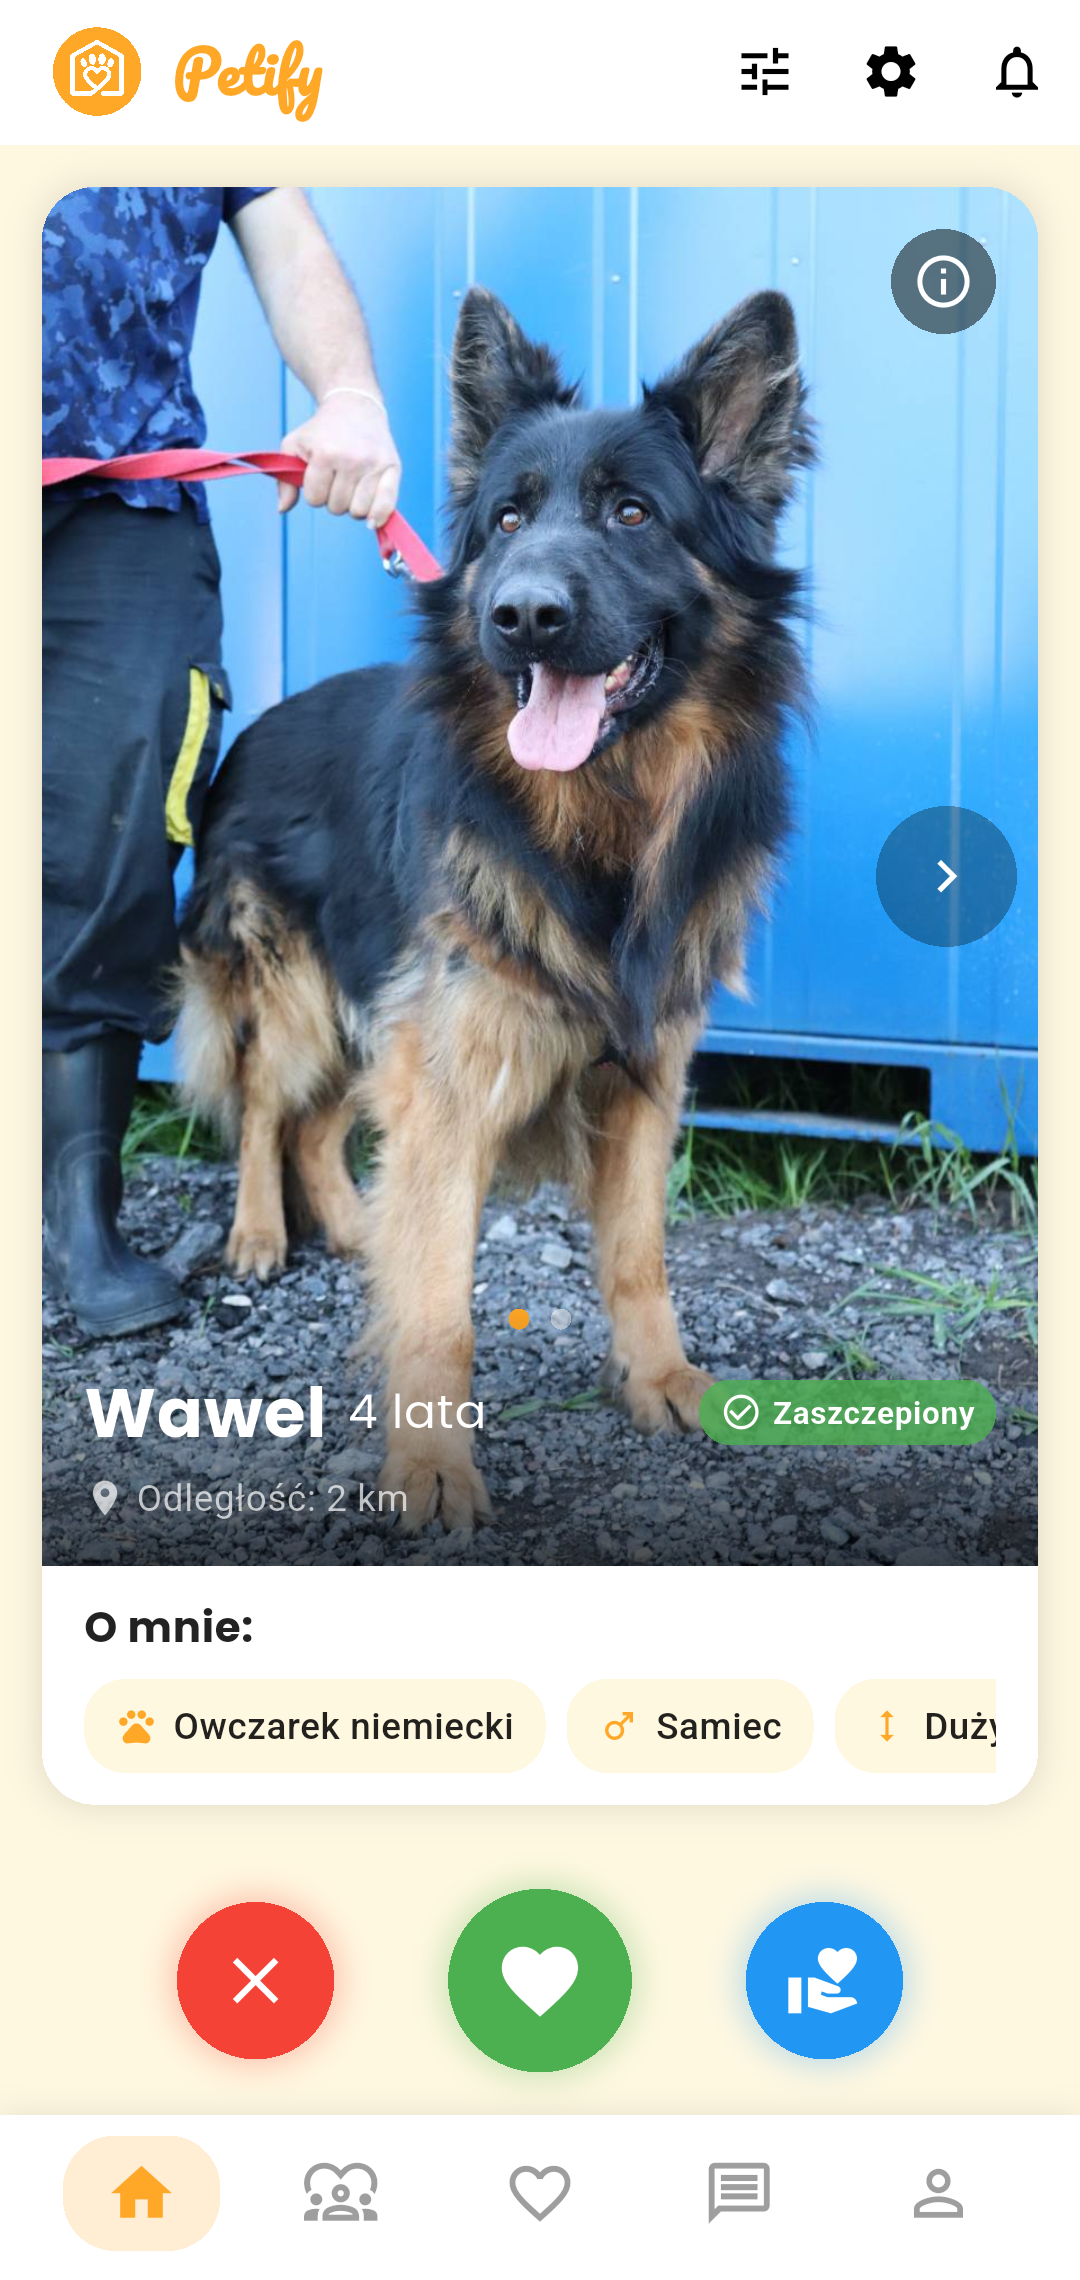
\includegraphics[width=\textwidth]{app-main.png}
\end{subfigure}
\begin{subfigure}{0.325\textwidth}
    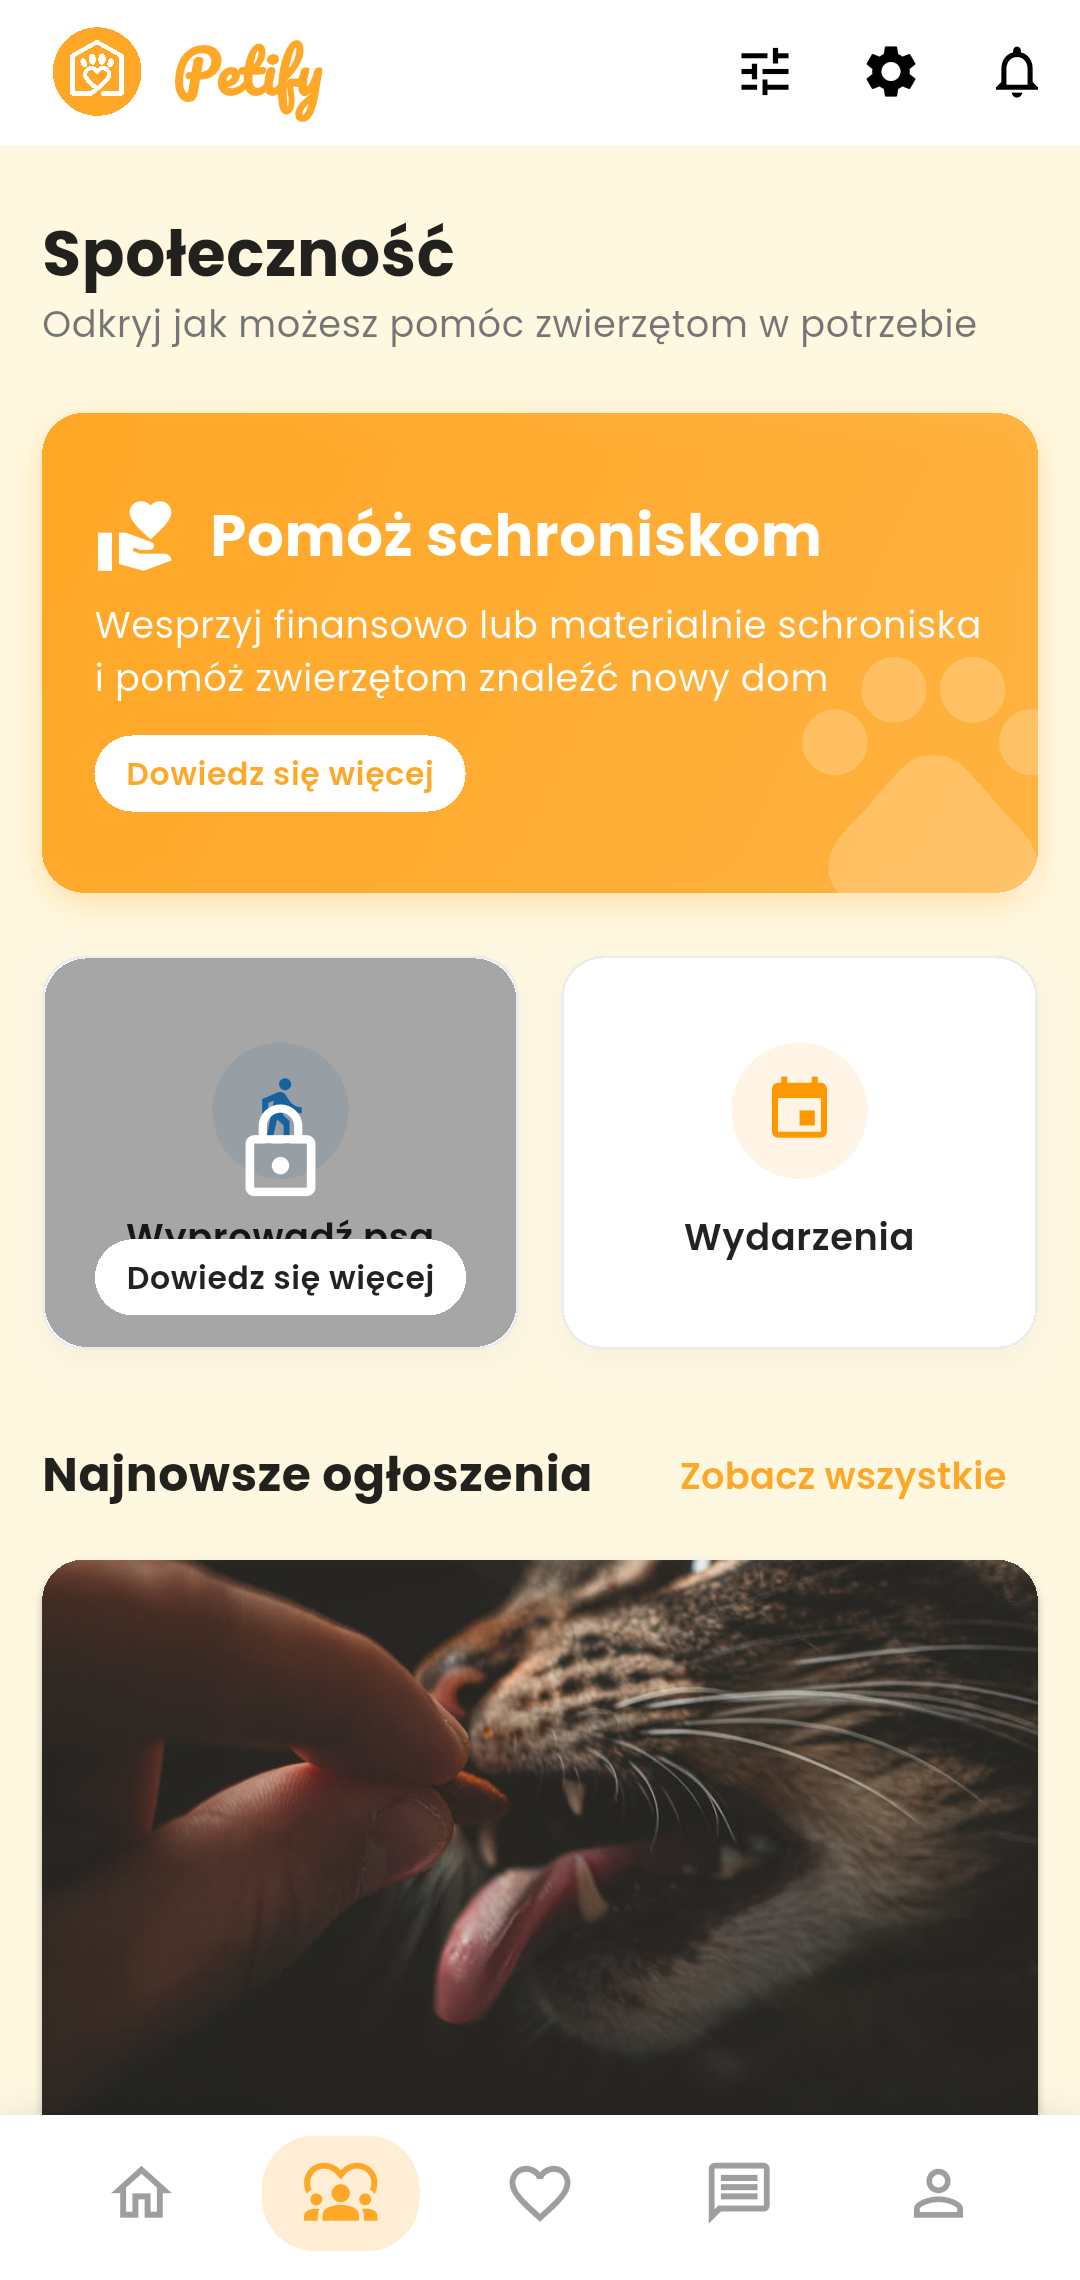
\includegraphics[width=\textwidth]{app-feed.png}
\end{subfigure}
\begin{subfigure}{0.325\textwidth}
    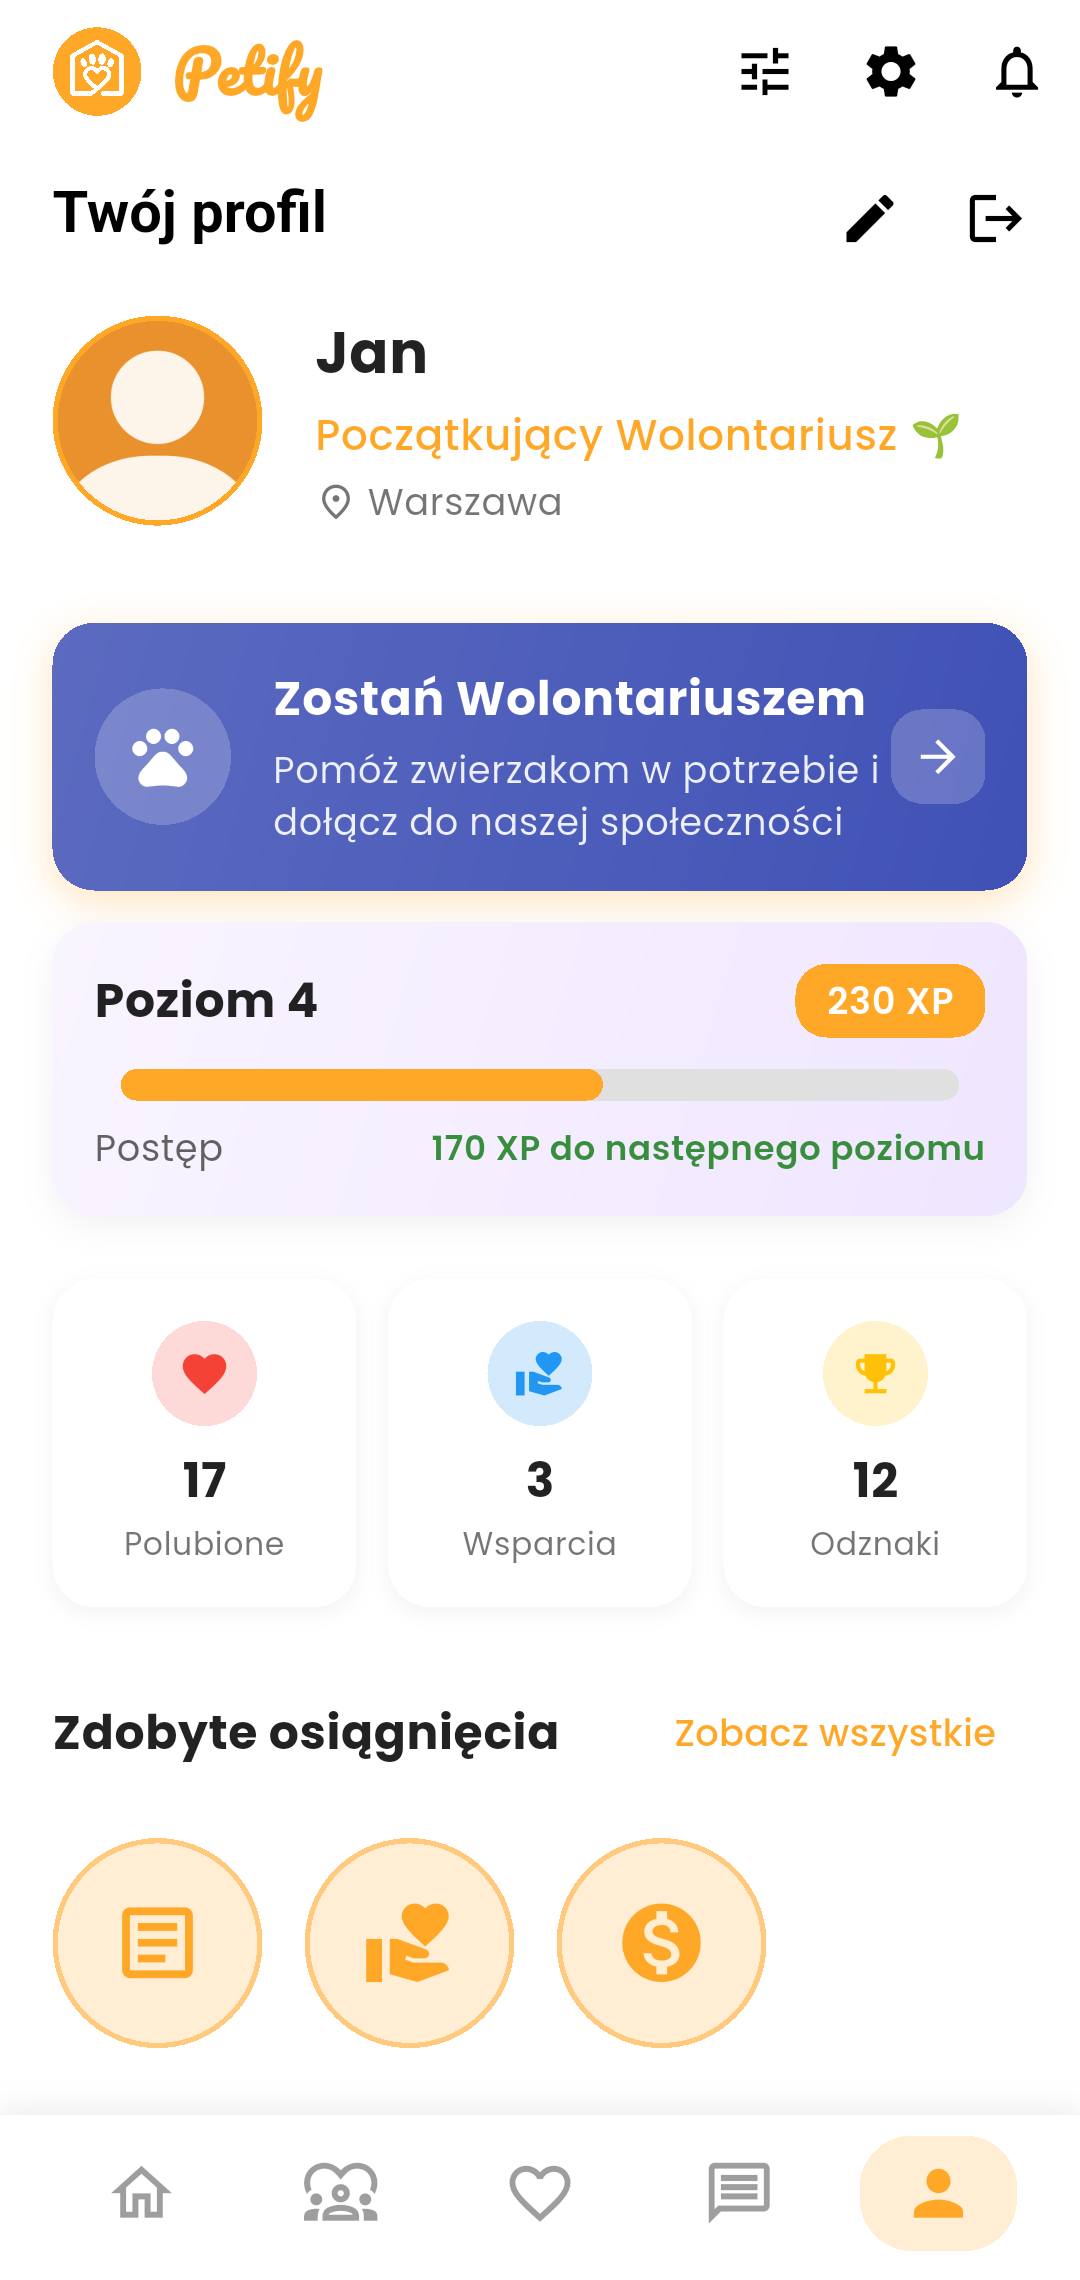
\includegraphics[width=\textwidth]{app-user.png}
\end{subfigure}
\caption{\centering Aplikacja mobilna: ekran główny z profilem zwierzęcia, sekcja~społeczności oraz profil użytkownika.}
\label{fig:example1}
\end{figure}
Zakładka ,,Społeczność'' prezentuje główny element zachęcający do finansowego wsparcia oraz kafelki z~nadchodzącymi wydarzeniami i~ogłoszeniami. Dzięki temu użytkownik może szybko dowiedzieć się o~potrzebach zwierząt i~lokalnych akcjach.

Profil użytkownika wyświetla zdjęcie, imię, miasto oraz poziom zaangażowania (,,Początkujący Wolontariusz'') z~paskiem punktów doświadczenia. Pod nim widoczne są statystyki: liczba polubionych zwierząt, dokonanych wsparć i~zdobytych odznak, co motywuje do dalszej aktywności.
\end{block}
\begin{block}{Podsumowanie}
\justifying
Petify skutecznie rozwiązuje problem niskiej adopcyjności zwierząt ze schronisk poprzez nowoczesne podejście do prezentacji i~wyszukiwania pupili. Aplikacja łączy intuicyjny interfejs mobilny z~zaawansowanym systemem zarządzania dla schronisk, tworząc kompleksową platformę wspierającą adopcję.
\end{block}
\begin{block}{Podziękowania}
Serdecznie~dziękujemy~firmie~Deloitte~Digital~za~nieocenione~wsparcie i profesjonalne doradztwo, które miało istotne znaczenie dla realizacji naszego projektu.
\end{block}
\end{column}
\end{columns}
    \vfill
\end{frame}
\end{document}
